\documentclass[twoside]{book}

% Packages required by doxygen
\usepackage{fixltx2e}
\usepackage{calc}
\usepackage{doxygen}
\usepackage[export]{adjustbox} % also loads graphicx
\usepackage{graphicx}
\usepackage[utf8]{inputenc}
\usepackage{makeidx}
\usepackage{multicol}
\usepackage{multirow}
\PassOptionsToPackage{warn}{textcomp}
\usepackage{textcomp}
\usepackage[nointegrals]{wasysym}
\usepackage[table]{xcolor}

% Font selection
\usepackage[T1]{fontenc}
\usepackage[scaled=.90]{helvet}
\usepackage{courier}
\usepackage{amssymb}
\usepackage{sectsty}
\renewcommand{\familydefault}{\sfdefault}
\allsectionsfont{%
  \fontseries{bc}\selectfont%
  \color{darkgray}%
}
\renewcommand{\DoxyLabelFont}{%
  \fontseries{bc}\selectfont%
  \color{darkgray}%
}
\newcommand{\+}{\discretionary{\mbox{\scriptsize$\hookleftarrow$}}{}{}}

% Page & text layout
\usepackage{geometry}
\geometry{%
  a4paper,%
  top=2.5cm,%
  bottom=2.5cm,%
  left=2.5cm,%
  right=2.5cm%
}
\tolerance=750
\hfuzz=15pt
\hbadness=750
\setlength{\emergencystretch}{15pt}
\setlength{\parindent}{0cm}
\setlength{\parskip}{3ex plus 2ex minus 2ex}
\makeatletter
\renewcommand{\paragraph}{%
  \@startsection{paragraph}{4}{0ex}{-1.0ex}{1.0ex}{%
    \normalfont\normalsize\bfseries\SS@parafont%
  }%
}
\renewcommand{\subparagraph}{%
  \@startsection{subparagraph}{5}{0ex}{-1.0ex}{1.0ex}{%
    \normalfont\normalsize\bfseries\SS@subparafont%
  }%
}
\makeatother

% Headers & footers
\usepackage{fancyhdr}
\pagestyle{fancyplain}
\fancyhead[LE]{\fancyplain{}{\bfseries\thepage}}
\fancyhead[CE]{\fancyplain{}{}}
\fancyhead[RE]{\fancyplain{}{\bfseries\leftmark}}
\fancyhead[LO]{\fancyplain{}{\bfseries\rightmark}}
\fancyhead[CO]{\fancyplain{}{}}
\fancyhead[RO]{\fancyplain{}{\bfseries\thepage}}
\fancyfoot[LE]{\fancyplain{}{}}
\fancyfoot[CE]{\fancyplain{}{}}
\fancyfoot[RE]{\fancyplain{}{\bfseries\scriptsize Generated by Doxygen }}
\fancyfoot[LO]{\fancyplain{}{\bfseries\scriptsize Generated by Doxygen }}
\fancyfoot[CO]{\fancyplain{}{}}
\fancyfoot[RO]{\fancyplain{}{}}
\renewcommand{\footrulewidth}{0.4pt}
\renewcommand{\chaptermark}[1]{%
  \markboth{#1}{}%
}
\renewcommand{\sectionmark}[1]{%
  \markright{\thesection\ #1}%
}

% Indices & bibliography
\usepackage{natbib}
\usepackage[titles]{tocloft}
\setcounter{tocdepth}{3}
\setcounter{secnumdepth}{5}
\makeindex

% Hyperlinks (required, but should be loaded last)
\usepackage{ifpdf}
\ifpdf
  \usepackage[pdftex,pagebackref=true]{hyperref}
\else
  \usepackage[ps2pdf,pagebackref=true]{hyperref}
\fi
\hypersetup{%
  colorlinks=true,%
  linkcolor=blue,%
  citecolor=blue,%
  unicode%
}

% Custom commands
\newcommand{\clearemptydoublepage}{%
  \newpage{\pagestyle{empty}\cleardoublepage}%
}

\usepackage{caption}
\captionsetup{labelsep=space,justification=centering,font={bf},singlelinecheck=off,skip=4pt,position=top}

%===== C O N T E N T S =====

\begin{document}

% Titlepage & ToC
\hypersetup{pageanchor=false,
             bookmarksnumbered=true,
             pdfencoding=unicode
            }
\pagenumbering{roman}
\begin{titlepage}
\vspace*{7cm}
\begin{center}%
{\Large My Project }\\
\vspace*{1cm}
{\large Generated by Doxygen 1.8.11}\\
\end{center}
\end{titlepage}
\clearemptydoublepage
\tableofcontents
\clearemptydoublepage
\pagenumbering{arabic}
\hypersetup{pageanchor=true}

%--- Begin generated contents ---
\chapter{Ka\+ZaA implementation}
\label{index}\hypertarget{index}{}\hypertarget{index_intro_sec}{}\section{Introduction}\label{index_intro_sec}
In the following project a p2p network has been implemented. Here overall project structure is described, detailed description of each structure is present below.\hypertarget{index_install_sec}{}\section{Installation}\label{index_install_sec}
First of all you need to clone project repository\+: \href{https://github.com/x3medima17/p2p}{\tt https\+://github.\+com/x3medima17/p2p}~\newline
Then you have to run cmake as follows \begin{quote}
cd build ~\newline
cmake ..~\newline
make~\newline
\end{quote}


It will generate {\ttfamily super} and {\ttfamily child} executables in {\ttfamily build} directory, and copy them to the following ones\+: \begin{quote}
env/child/child1/~\newline
env/child/child2/~\newline
env/child/child3/~\newline
env/child/super/~\newline
\end{quote}


Now you are ready to run those files, each child has its own {\ttfamily data} and {\ttfamily download} directory.\hypertarget{index_serv}{}\section{Server}\label{index_serv}
Both Child and Super are based on client-\/server architecture, and both of them can work as clients and servers at the same time.~\newline
For this purpose a listener server is needed on each side, the architecture that I have chosen is \hyperlink{classIOLoop}{I\+O\+Loop} \hypertarget{index_ioloop}{}\subsection{I\+O\+Loop}\label{index_ioloop}
\hyperlink{classIOLoop}{I\+O\+Loop} is an class that uses IO Multiplexing, it has a listener socket and continuously loops waiting waiting for incoming data. Using {\ttfamily select()} it accepts and spawns new sockets. ~\newline
It has a \hyperlink{classIOHandler}{I\+O\+Handler} virtual class that is used to handle incoming data.

iohandler \hyperlink{classIOHandler}{I\+O\+Handler} \hyperlink{classIOHandler}{I\+O\+Handler} is an semi-\/abstract class that is a member of \hyperlink{classIOLoop}{I\+O\+Loop}, its job is to take incoming data and do some actions on it. Its default behaivor is to ignore any data.\hypertarget{index_siohandler}{}\subsection{Super\+I\+O\+Handler}\label{index_siohandler}
\hyperlink{classSuperIOHandler}{Super\+I\+O\+Handler} extends \hyperlink{classIOHandler}{I\+O\+Handler} and is passed to \hyperlink{classIOLoop}{I\+O\+Loop}, this way Supers\textquotesingle{}s \hyperlink{classIOLoop}{I\+O\+Loop} will invoke \hyperlink{classSuperIOHandler}{Super\+I\+O\+Handler}\textquotesingle{}s on\+Read method.\hypertarget{index_ciohadnler}{}\subsection{Child\+I\+O\+Handler}\label{index_ciohadnler}
\hyperlink{classSuperIOHandler}{Super\+I\+O\+Handler} extends \hyperlink{classIOHandler}{I\+O\+Handler} and is passed to \hyperlink{classIOLoop}{I\+O\+Loop}, this way Supers\textquotesingle{}s \hyperlink{classIOLoop}{I\+O\+Loop} will invoke \hyperlink{classSuperIOHandler}{Super\+I\+O\+Handler}\textquotesingle{}s on\+Read method.\hypertarget{index_Super}{}\section{Super}\label{index_Super}
It is source code of Super \hyperlink{structNode}{Node}, first of all it scans command line arguments. If another supernode arguments are present it it will send H\+E\+L\+L\+O\+\_\+\+S\+U\+P\+ER message (messages are explained later), then it takes its own port and starts server using \hyperlink{classIOLoop}{I\+O\+Loop} on that port.\hypertarget{index_Child}{}\section{Child}\label{index_Child}
It is source code of Child \hyperlink{structNode}{Node}, first of all it scans command line arguments. it finds supernode arguments and sends H\+E\+L\+L\+O\+\_\+\+C\+H\+I\+LD message (messages are explained later), then it takes its own port and starts server using \hyperlink{classIOLoop}{I\+O\+Loop} on that port. 
\chapter{Namespace Index}
\section{Namespace List}
Here is a list of all documented namespaces with brief descriptions\+:\begin{DoxyCompactList}
\item\contentsline{section}{\hyperlink{namespaceUtils}{Utils} }{\pageref{namespaceUtils}}{}
\end{DoxyCompactList}

\chapter{Hierarchical Index}
\section{Class Hierarchy}
This inheritance list is sorted roughly, but not completely, alphabetically\+:\begin{DoxyCompactList}
\item \contentsline{section}{File}{\pageref{structFile}}{}
\item \contentsline{section}{File\+Table}{\pageref{classFileTable}}{}
\item \contentsline{section}{I\+O\+Handler}{\pageref{classIOHandler}}{}
\begin{DoxyCompactList}
\item \contentsline{section}{Child\+I\+O\+Handler}{\pageref{classChildIOHandler}}{}
\item \contentsline{section}{Super\+I\+O\+Handler}{\pageref{classSuperIOHandler}}{}
\end{DoxyCompactList}
\item \contentsline{section}{I\+O\+Loop}{\pageref{classIOLoop}}{}
\item \contentsline{section}{Message}{\pageref{structMessage}}{}
\item \contentsline{section}{Node}{\pageref{structNode}}{}
\item \contentsline{section}{Socket}{\pageref{classSocket}}{}
\end{DoxyCompactList}

\chapter{Class Index}
\section{Class List}
Here are the classes, structs, unions and interfaces with brief descriptions\+:\begin{DoxyCompactList}
\item\contentsline{section}{\hyperlink{classChildIOHandler}{Child\+I\+O\+Handler} }{\pageref{classChildIOHandler}}{}
\item\contentsline{section}{\hyperlink{structFile}{File} }{\pageref{structFile}}{}
\item\contentsline{section}{\hyperlink{classFileTable}{File\+Table} }{\pageref{classFileTable}}{}
\item\contentsline{section}{\hyperlink{classIOHandler}{I\+O\+Handler} }{\pageref{classIOHandler}}{}
\item\contentsline{section}{\hyperlink{classIOLoop}{I\+O\+Loop} }{\pageref{classIOLoop}}{}
\item\contentsline{section}{\hyperlink{structMessage}{Message} }{\pageref{structMessage}}{}
\item\contentsline{section}{\hyperlink{structNode}{Node} }{\pageref{structNode}}{}
\item\contentsline{section}{\hyperlink{classSocket}{Socket} }{\pageref{classSocket}}{}
\item\contentsline{section}{\hyperlink{classSuperIOHandler}{Super\+I\+O\+Handler} }{\pageref{classSuperIOHandler}}{}
\end{DoxyCompactList}

\chapter{Namespace Documentation}
\hypertarget{namespaceUtils}{}\section{Utils Namespace Reference}
\label{namespaceUtils}\index{Utils@{Utils}}
\subsection*{Functions}
\begin{DoxyCompactItemize}
\item 
uint32\+\_\+t \hyperlink{namespaceUtils_a61c151a32493475c413d3b7964615d01}{uint32\+\_\+from\+\_\+vec} (std\+::vector$<$ uint8\+\_\+t $>$\+::const\+\_\+iterator it)
\item 
std\+::vector$<$ uint8\+\_\+t $>$ \hyperlink{namespaceUtils_a268ccd9cd3521e318e67a4c58cb95066}{vec\+\_\+from\+\_\+uint32} (uint32\+\_\+t val)
\item 
\hyperlink{structMessage}{Message} \hyperlink{namespaceUtils_a632dc21b737a7e31b5d5653d8fb927c6}{read\+\_\+message} (const \hyperlink{classSocket}{Socket} \&sock, size\+\_\+t timeout=5000)
\item 
void \hyperlink{namespaceUtils_a3a16defae746b5d1ef3f072da17ac377}{write\+\_\+message} (const \hyperlink{classSocket}{Socket} \&sock, \hyperlink{structMessage}{Message} \&msg)
\item 
std\+::map$<$ std\+::string, std\+::string $>$ \hyperlink{namespaceUtils_a50030bbcd5a72967f903913b18ac11dd}{parse\+\_\+cmd\+\_\+args} (int argc, char $\ast$$\ast$argv)
\item 
uint16\+\_\+t {\bfseries uint16\+\_\+from\+\_\+vec} (std\+::vector$<$ uint8\+\_\+t $>$\+::const\+\_\+iterator it)\hypertarget{namespaceUtils_a9aefb9599b00ed911043880504b3cc50}{}\label{namespaceUtils_a9aefb9599b00ed911043880504b3cc50}

\end{DoxyCompactItemize}
\subsection*{Variables}
\begin{DoxyCompactItemize}
\item 
const size\+\_\+t \hyperlink{namespaceUtils_aa3bfa39b8378ffaa8f0452645d5dd44f}{H\+E\+A\+D\+E\+R\+\_\+\+S\+I\+ZE} \{12\}
\end{DoxyCompactItemize}


\subsection{Detailed Description}
Utility namespace that contains all necessary function and constants 

\subsection{Function Documentation}
\index{Utils@{Utils}!parse\+\_\+cmd\+\_\+args@{parse\+\_\+cmd\+\_\+args}}
\index{parse\+\_\+cmd\+\_\+args@{parse\+\_\+cmd\+\_\+args}!Utils@{Utils}}
\subsubsection[{\texorpdfstring{parse\+\_\+cmd\+\_\+args(int argc, char $\ast$$\ast$argv)}{parse_cmd_args(int argc, char **argv)}}]{\setlength{\rightskip}{0pt plus 5cm}std\+::map$<$ std\+::string, std\+::string $>$ Utils\+::parse\+\_\+cmd\+\_\+args (
\begin{DoxyParamCaption}
\item[{int}]{argc, }
\item[{char $\ast$$\ast$}]{argv}
\end{DoxyParamCaption}
)}\hypertarget{namespaceUtils_a50030bbcd5a72967f903913b18ac11dd}{}\label{namespaceUtils_a50030bbcd5a72967f903913b18ac11dd}
This function is invoken in Child and Super it parses command line 
\begin{DoxyParams}{Parameters}
{\em argc} & Number of arguments \\
\hline
{\em argv} & Pointer to $\ast$char (arguments) \\
\hline
\end{DoxyParams}
\begin{DoxyReturn}{Returns}
Returns a map of string(argument) -\/$>$ string(value) 
\end{DoxyReturn}
\index{Utils@{Utils}!read\+\_\+message@{read\+\_\+message}}
\index{read\+\_\+message@{read\+\_\+message}!Utils@{Utils}}
\subsubsection[{\texorpdfstring{read\+\_\+message(const Socket \&sock, size\+\_\+t timeout=5000)}{read_message(const Socket &sock, size_t timeout=5000)}}]{\setlength{\rightskip}{0pt plus 5cm}{\bf Message} Utils\+::read\+\_\+message (
\begin{DoxyParamCaption}
\item[{const {\bf Socket} \&}]{sock, }
\item[{size\+\_\+t}]{timeout = {\ttfamily 5000}}
\end{DoxyParamCaption}
)}\hypertarget{namespaceUtils_a632dc21b737a7e31b5d5653d8fb927c6}{}\label{namespaceUtils_a632dc21b737a7e31b5d5653d8fb927c6}
Most used function in the app, it reads a \hyperlink{structMessage}{Message} from the socket 
\begin{DoxyParams}{Parameters}
{\em sock} & Constant socket reference \\
\hline
{\em timeout} & Timeout of reading (required in the task), it has a default value \\
\hline
\end{DoxyParams}
\begin{DoxyReturn}{Returns}
It return a \hyperlink{structMessage}{Message} instance 
\end{DoxyReturn}
\index{Utils@{Utils}!uint32\+\_\+from\+\_\+vec@{uint32\+\_\+from\+\_\+vec}}
\index{uint32\+\_\+from\+\_\+vec@{uint32\+\_\+from\+\_\+vec}!Utils@{Utils}}
\subsubsection[{\texorpdfstring{uint32\+\_\+from\+\_\+vec(std\+::vector$<$ uint8\+\_\+t $>$\+::const\+\_\+iterator it)}{uint32_from_vec(std::vector< uint8_t >::const_iterator it)}}]{\setlength{\rightskip}{0pt plus 5cm}uint32\+\_\+t Utils\+::uint32\+\_\+from\+\_\+vec (
\begin{DoxyParamCaption}
\item[{std\+::vector$<$ uint8\+\_\+t $>$\+::const\+\_\+iterator}]{it}
\end{DoxyParamCaption}
)}\hypertarget{namespaceUtils_a61c151a32493475c413d3b7964615d01}{}\label{namespaceUtils_a61c151a32493475c413d3b7964615d01}
Method that transforms a byte array to 4 byte integer 
\begin{DoxyParams}{Parameters}
{\em it} & Vectors iterator \\
\hline
\end{DoxyParams}
\begin{DoxyReturn}{Returns}
unsigned int value 
\end{DoxyReturn}
\index{Utils@{Utils}!vec\+\_\+from\+\_\+uint32@{vec\+\_\+from\+\_\+uint32}}
\index{vec\+\_\+from\+\_\+uint32@{vec\+\_\+from\+\_\+uint32}!Utils@{Utils}}
\subsubsection[{\texorpdfstring{vec\+\_\+from\+\_\+uint32(uint32\+\_\+t val)}{vec_from_uint32(uint32_t val)}}]{\setlength{\rightskip}{0pt plus 5cm}std\+::vector$<$ uint8\+\_\+t $>$ Utils\+::vec\+\_\+from\+\_\+uint32 (
\begin{DoxyParamCaption}
\item[{uint32\+\_\+t}]{val}
\end{DoxyParamCaption}
)}\hypertarget{namespaceUtils_a268ccd9cd3521e318e67a4c58cb95066}{}\label{namespaceUtils_a268ccd9cd3521e318e67a4c58cb95066}
Same as previous but does exactly the oposite action 
\begin{DoxyParams}{Parameters}
{\em val} & unsiged int \\
\hline
\end{DoxyParams}
\begin{DoxyReturn}{Returns}
vector of bytes 
\end{DoxyReturn}
\index{Utils@{Utils}!write\+\_\+message@{write\+\_\+message}}
\index{write\+\_\+message@{write\+\_\+message}!Utils@{Utils}}
\subsubsection[{\texorpdfstring{write\+\_\+message(const Socket \&sock, Message \&msg)}{write_message(const Socket &sock, Message &msg)}}]{\setlength{\rightskip}{0pt plus 5cm}void Utils\+::write\+\_\+message (
\begin{DoxyParamCaption}
\item[{const {\bf Socket} \&}]{sock, }
\item[{{\bf Message} \&}]{msg}
\end{DoxyParamCaption}
)}\hypertarget{namespaceUtils_a3a16defae746b5d1ef3f072da17ac377}{}\label{namespaceUtils_a3a16defae746b5d1ef3f072da17ac377}
This method writes a \hyperlink{structMessage}{Message} into \hyperlink{classSocket}{Socket} 
\begin{DoxyParams}{Parameters}
{\em sock} & Constant \hyperlink{classSocket}{Socket} reference \\
\hline
{\em msg} & \\
\hline
\end{DoxyParams}


\subsection{Variable Documentation}
\index{Utils@{Utils}!H\+E\+A\+D\+E\+R\+\_\+\+S\+I\+ZE@{H\+E\+A\+D\+E\+R\+\_\+\+S\+I\+ZE}}
\index{H\+E\+A\+D\+E\+R\+\_\+\+S\+I\+ZE@{H\+E\+A\+D\+E\+R\+\_\+\+S\+I\+ZE}!Utils@{Utils}}
\subsubsection[{\texorpdfstring{H\+E\+A\+D\+E\+R\+\_\+\+S\+I\+ZE}{HEADER_SIZE}}]{\setlength{\rightskip}{0pt plus 5cm}const size\+\_\+t Utils\+::\+H\+E\+A\+D\+E\+R\+\_\+\+S\+I\+ZE \{12\}}\hypertarget{namespaceUtils_aa3bfa39b8378ffaa8f0452645d5dd44f}{}\label{namespaceUtils_aa3bfa39b8378ffaa8f0452645d5dd44f}
Header size of message 
\chapter{Class Documentation}
\hypertarget{classChildIOHandler}{}\section{Child\+I\+O\+Handler Class Reference}
\label{classChildIOHandler}\index{Child\+I\+O\+Handler@{Child\+I\+O\+Handler}}


Inheritance diagram for Child\+I\+O\+Handler\+:\nopagebreak
\begin{figure}[H]
\begin{center}
\leavevmode
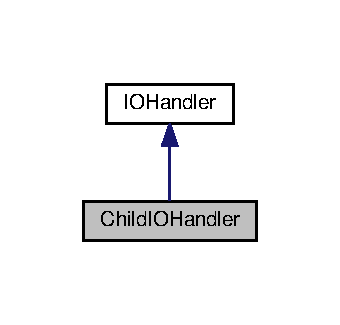
\includegraphics[width=163pt]{classChildIOHandler__inherit__graph}
\end{center}
\end{figure}


Collaboration diagram for Child\+I\+O\+Handler\+:\nopagebreak
\begin{figure}[H]
\begin{center}
\leavevmode
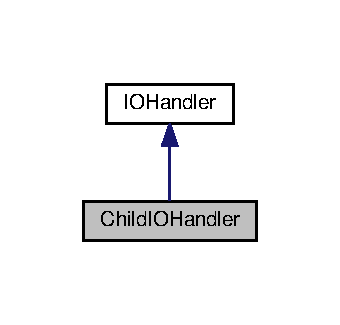
\includegraphics[width=163pt]{classChildIOHandler__coll__graph}
\end{center}
\end{figure}
\subsection*{Public Member Functions}
\begin{DoxyCompactItemize}
\item 
void {\bfseries on\+Read} (size\+\_\+t fd, fd\+\_\+set $\ast$readfd) override\hypertarget{classChildIOHandler_a9838d8ec92e09028459171f834371f0f}{}\label{classChildIOHandler_a9838d8ec92e09028459171f834371f0f}

\item 
void {\bfseries on\+Read} (std\+::shared\+\_\+ptr$<$ \hyperlink{classSocket}{Socket} $>$ \&client, fd\+\_\+set $\ast$readfd) override\hypertarget{classChildIOHandler_acd3941962eb3d34505348be79f151334}{}\label{classChildIOHandler_acd3941962eb3d34505348be79f151334}

\end{DoxyCompactItemize}


The documentation for this class was generated from the following file\+:\begin{DoxyCompactItemize}
\item 
child.\+cpp\end{DoxyCompactItemize}

\hypertarget{structFile}{}\section{File Struct Reference}
\label{structFile}\index{File@{File}}


{\ttfamily \#include $<$File.\+hpp$>$}

\subsection*{Public Member Functions}
\begin{DoxyCompactItemize}
\item 
\hyperlink{structFile_ad0746cf10905ee35809f9e64452dc947}{File} (std\+::string fname, size\+\_\+t size)
\item 
void \hyperlink{structFile_a953519811424483b08848c889a7f0743}{print} () const 
\end{DoxyCompactItemize}
\subsection*{Public Attributes}
\begin{DoxyCompactItemize}
\item 
std\+::string {\bfseries fname\+\_\+}\hypertarget{structFile_ac40ef1df4d43c2dee0086ea073e5b1fd}{}\label{structFile_ac40ef1df4d43c2dee0086ea073e5b1fd}

\item 
size\+\_\+t {\bfseries size\+\_\+}\hypertarget{structFile_ac884c55c119bb40a06be3f81abaa79ab}{}\label{structFile_ac884c55c119bb40a06be3f81abaa79ab}

\end{DoxyCompactItemize}


\subsection{Detailed Description}
Child uses C++17 feature called File\+System, in order to keep data close I use \hyperlink{structFile}{File} class, it stores filename and size. 

\subsection{Constructor \& Destructor Documentation}
\index{File@{File}!File@{File}}
\index{File@{File}!File@{File}}
\subsubsection[{\texorpdfstring{File(std\+::string fname, size\+\_\+t size)}{File(std::string fname, size_t size)}}]{\setlength{\rightskip}{0pt plus 5cm}File\+::\+File (
\begin{DoxyParamCaption}
\item[{std\+::string}]{fname, }
\item[{size\+\_\+t}]{size}
\end{DoxyParamCaption}
)}\hypertarget{structFile_ad0746cf10905ee35809f9e64452dc947}{}\label{structFile_ad0746cf10905ee35809f9e64452dc947}
Standard file constructor 
\begin{DoxyParams}{Parameters}
{\em fname} & \hyperlink{structFile}{File} name \\
\hline
{\em size} & \hyperlink{structFile}{File} size \\
\hline
\end{DoxyParams}


\subsection{Member Function Documentation}
\index{File@{File}!print@{print}}
\index{print@{print}!File@{File}}
\subsubsection[{\texorpdfstring{print() const }{print() const }}]{\setlength{\rightskip}{0pt plus 5cm}void File\+::print (
\begin{DoxyParamCaption}
{}
\end{DoxyParamCaption}
) const}\hypertarget{structFile_a953519811424483b08848c889a7f0743}{}\label{structFile_a953519811424483b08848c889a7f0743}
Method that prints file data in a pretty format. Mainly used for debugging. 

The documentation for this struct was generated from the following files\+:\begin{DoxyCompactItemize}
\item 
include/File.\+hpp\item 
src/File.\+cpp\end{DoxyCompactItemize}

\hypertarget{classFileTable}{}\section{File\+Table Class Reference}
\label{classFileTable}\index{File\+Table@{File\+Table}}
\subsection*{Public Member Functions}
\begin{DoxyCompactItemize}
\item 
void {\bfseries insert} (std\+::string fname, size\+\_\+t fsize, std\+::string ip, uint16\+\_\+t port)\hypertarget{classFileTable_a7d5b184a90260b6272e6afa1e719c6b8}{}\label{classFileTable_a7d5b184a90260b6272e6afa1e719c6b8}

\item 
std\+::map$<$ std\+::string, Entry $>$\+::const\+\_\+iterator {\bfseries find} (std\+::string fname)\hypertarget{classFileTable_a9e4e2ab0bc0f248a12656ff97000e9ad}{}\label{classFileTable_a9e4e2ab0bc0f248a12656ff97000e9ad}

\item 
size\+\_\+t {\bfseries size} ()\hypertarget{classFileTable_a80a5e2ecc2229bb02a451f66d5cb3e87}{}\label{classFileTable_a80a5e2ecc2229bb02a451f66d5cb3e87}

\item 
std\+::map$<$ std\+::string, Entry $>$\+::const\+\_\+iterator {\bfseries beign} ()\hypertarget{classFileTable_a173fc365feb6a20c8531f8c731bcc7c4}{}\label{classFileTable_a173fc365feb6a20c8531f8c731bcc7c4}

\item 
std\+::map$<$ std\+::string, Entry $>$\+::const\+\_\+iterator {\bfseries end} ()\hypertarget{classFileTable_aae5fdbef3e406b6a2a475ca74dc8f75a}{}\label{classFileTable_aae5fdbef3e406b6a2a475ca74dc8f75a}

\item 
void {\bfseries print} ()\hypertarget{classFileTable_ab9b62d0b7cd222d55f92ce7f6991a77b}{}\label{classFileTable_ab9b62d0b7cd222d55f92ce7f6991a77b}

\end{DoxyCompactItemize}


The documentation for this class was generated from the following file\+:\begin{DoxyCompactItemize}
\item 
super.\+cpp\end{DoxyCompactItemize}

\hypertarget{classIOHandler}{}\section{I\+O\+Handler Class Reference}
\label{classIOHandler}\index{I\+O\+Handler@{I\+O\+Handler}}


Inheritance diagram for I\+O\+Handler\+:\nopagebreak
\begin{figure}[H]
\begin{center}
\leavevmode
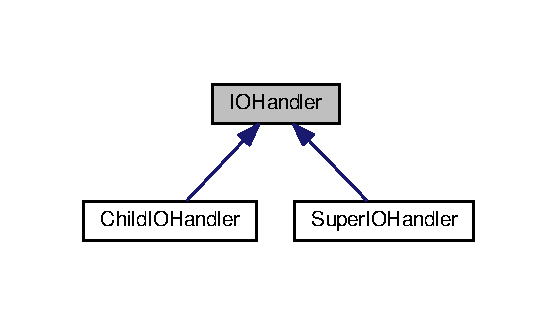
\includegraphics[width=268pt]{classIOHandler__inherit__graph}
\end{center}
\end{figure}
\subsection*{Public Member Functions}
\begin{DoxyCompactItemize}
\item 
virtual void {\bfseries on\+Read} (size\+\_\+t fd, fd\+\_\+set $\ast$readfd)\hypertarget{classIOHandler_a623e46574ae279609c2f1f3020890c92}{}\label{classIOHandler_a623e46574ae279609c2f1f3020890c92}

\item 
virtual void {\bfseries on\+Read} (std\+::shared\+\_\+ptr$<$ \hyperlink{classSocket}{Socket} $>$ \&client, fd\+\_\+set $\ast$readfd)\hypertarget{classIOHandler_ac3d156d3c2051e6cc19256ad20111d52}{}\label{classIOHandler_ac3d156d3c2051e6cc19256ad20111d52}

\end{DoxyCompactItemize}


The documentation for this class was generated from the following files\+:\begin{DoxyCompactItemize}
\item 
include/I\+O\+Handler.\+hpp\item 
src/I\+O\+Handler.\+cpp\end{DoxyCompactItemize}

\hypertarget{classIOLoop}{}\section{I\+O\+Loop Class Reference}
\label{classIOLoop}\index{I\+O\+Loop@{I\+O\+Loop}}
\subsection*{Public Member Functions}
\begin{DoxyCompactItemize}
\item 
{\bfseries I\+O\+Loop} (\hyperlink{classSocket}{Socket} \&, \hyperlink{classIOHandler}{I\+O\+Handler} \&)\hypertarget{classIOLoop_a991895206fdd315c28a9437d0b00e2a3}{}\label{classIOLoop_a991895206fdd315c28a9437d0b00e2a3}

\item 
void {\bfseries start} ()\hypertarget{classIOLoop_a227cd89b27b6f9cb302bf501943e2184}{}\label{classIOLoop_a227cd89b27b6f9cb302bf501943e2184}

\end{DoxyCompactItemize}


The documentation for this class was generated from the following files\+:\begin{DoxyCompactItemize}
\item 
include/I\+O\+Loop.\+hpp\item 
src/I\+O\+Loop.\+cpp\end{DoxyCompactItemize}

\hypertarget{structMessage}{}\section{Message Struct Reference}
\label{structMessage}\index{Message@{Message}}


{\ttfamily \#include $<$Message.\+hpp$>$}

\subsection*{Public Types}
\begin{DoxyCompactItemize}
\item 
enum \hyperlink{structMessage_a2cd191f475dd51cf44f57950e8862cd3}{M\+S\+G\+\_\+\+T\+Y\+P\+ES} \+: std\+::uint32\+\_\+t \{ \\*
{\bfseries C\+H\+I\+L\+D\+\_\+\+H\+E\+L\+LO} = 0x10, 
{\bfseries S\+U\+P\+E\+R\+\_\+\+H\+E\+L\+LO} = 0x11, 
{\bfseries S\+U\+P\+E\+R\+\_\+\+S\+U\+P\+E\+R\+\_\+\+H\+E\+L\+LO} = 0x12, 
{\bfseries F\+I\+L\+E\+\_\+\+I\+N\+FO} = 0x20, 
\\*
{\bfseries F\+I\+L\+E\+\_\+\+I\+N\+F\+O\+\_\+\+R\+E\+C\+V\+\_\+\+S\+U\+C\+C\+E\+SS} = 0x21, 
{\bfseries F\+I\+L\+E\+\_\+\+I\+N\+F\+O\+\_\+\+R\+E\+C\+V\+\_\+\+E\+R\+R\+OR} = 0x22, 
{\bfseries S\+E\+A\+R\+C\+H\+\_\+\+Q\+U\+E\+RY} = 0x30, 
{\bfseries S\+E\+A\+R\+C\+H\+\_\+\+A\+N\+S\+\_\+\+S\+U\+C\+C\+E\+SS} = 0x31, 
\\*
{\bfseries S\+E\+A\+R\+C\+H\+\_\+\+A\+N\+S\+\_\+\+F\+A\+IL} = 0x32, 
{\bfseries F\+I\+L\+E\+\_\+\+R\+EQ} = 0x40, 
{\bfseries F\+I\+L\+E\+\_\+\+R\+E\+S\+\_\+\+S\+U\+C\+C\+E\+SS} = 0x41, 
{\bfseries F\+I\+L\+E\+\_\+\+R\+E\+S\+\_\+\+F\+A\+IL} = 0x42, 
\\*
{\bfseries F\+I\+L\+E\+\_\+\+I\+N\+F\+O\+\_\+\+S\+H\+A\+RE} = 0x50, 
{\bfseries F\+I\+L\+E\+\_\+\+I\+N\+F\+O\+\_\+\+S\+H\+A\+R\+E\+\_\+\+S\+U\+C\+C\+E\+SS} = 0x51, 
{\bfseries F\+I\+L\+E\+\_\+\+I\+N\+F\+O\+\_\+\+S\+H\+A\+R\+E\+\_\+\+E\+R\+R\+OR} = 0x52
 \}
\end{DoxyCompactItemize}
\subsection*{Public Member Functions}
\begin{DoxyCompactItemize}
\item 
void \hyperlink{structMessage_a8c71bc14df10d1bc4a11c9912ec83e11}{set\+\_\+payload} (std\+::string s)
\item 
void \hyperlink{structMessage_a2967b7c13fd34ea7767b6e00076b3e76}{print} () const 
\end{DoxyCompactItemize}
\subsection*{Public Attributes}
\begin{DoxyCompactItemize}
\item 
uint32\+\_\+t {\bfseries total\+\_\+length} \{0\}\hypertarget{structMessage_a956485001345f455ac9ff675c9ec33ff}{}\label{structMessage_a956485001345f455ac9ff675c9ec33ff}

\item 
uint32\+\_\+t {\bfseries payload\+\_\+length} \{0\}\hypertarget{structMessage_a7540c3196a9649f76747a2e559ec34ac}{}\label{structMessage_a7540c3196a9649f76747a2e559ec34ac}

\item 
uint32\+\_\+t {\bfseries id} \{0\}\hypertarget{structMessage_a4c34674ebe8e9ac6a62a5b7c9c3e4123}{}\label{structMessage_a4c34674ebe8e9ac6a62a5b7c9c3e4123}

\item 
uint32\+\_\+t {\bfseries msg\+\_\+type} \{0\}\hypertarget{structMessage_a127a7296f3fe3ca2379b52d4d578d128}{}\label{structMessage_a127a7296f3fe3ca2379b52d4d578d128}

\item 
std\+::vector$<$ uint8\+\_\+t $>$ {\bfseries payload}\hypertarget{structMessage_ae178876b7de2f7d7629663350d20c599}{}\label{structMessage_ae178876b7de2f7d7629663350d20c599}

\item 
std\+::stringstream {\bfseries ss}\hypertarget{structMessage_ac499b4fb6c41a7512584c3cff3c68469}{}\label{structMessage_ac499b4fb6c41a7512584c3cff3c68469}

\end{DoxyCompactItemize}


\subsection{Detailed Description}
This is one the main classes in the application. All data exchange on the network is done through Messages. ~\newline
It has a header and a payload. Header is 12 bytes and payload has variable length. All payload is sent in a raw format and then read as string streams, the only exceptions are files that are being transmitted. 

\subsection{Member Enumeration Documentation}
\index{Message@{Message}!M\+S\+G\+\_\+\+T\+Y\+P\+ES@{M\+S\+G\+\_\+\+T\+Y\+P\+ES}}
\index{M\+S\+G\+\_\+\+T\+Y\+P\+ES@{M\+S\+G\+\_\+\+T\+Y\+P\+ES}!Message@{Message}}
\subsubsection[{\texorpdfstring{M\+S\+G\+\_\+\+T\+Y\+P\+ES}{MSG_TYPES}}]{\setlength{\rightskip}{0pt plus 5cm}enum {\bf Message\+::\+M\+S\+G\+\_\+\+T\+Y\+P\+ES} \+: std\+::uint32\+\_\+t\hspace{0.3cm}{\ttfamily [strong]}}\hypertarget{structMessage_a2cd191f475dd51cf44f57950e8862cd3}{}\label{structMessage_a2cd191f475dd51cf44f57950e8862cd3}
Enum designed to work safely with \hyperlink{structMessage}{Message} types No raw flags are used, only encapsulated enum 

\subsection{Member Function Documentation}
\index{Message@{Message}!print@{print}}
\index{print@{print}!Message@{Message}}
\subsubsection[{\texorpdfstring{print() const }{print() const }}]{\setlength{\rightskip}{0pt plus 5cm}void Message\+::print (
\begin{DoxyParamCaption}
{}
\end{DoxyParamCaption}
) const}\hypertarget{structMessage_a2967b7c13fd34ea7767b6e00076b3e76}{}\label{structMessage_a2967b7c13fd34ea7767b6e00076b3e76}
Method that prints message in a pretty format. Mainly used for debugging. \index{Message@{Message}!set\+\_\+payload@{set\+\_\+payload}}
\index{set\+\_\+payload@{set\+\_\+payload}!Message@{Message}}
\subsubsection[{\texorpdfstring{set\+\_\+payload(std\+::string s)}{set_payload(std::string s)}}]{\setlength{\rightskip}{0pt plus 5cm}void Message\+::set\+\_\+payload (
\begin{DoxyParamCaption}
\item[{std\+::string}]{s}
\end{DoxyParamCaption}
)}\hypertarget{structMessage_a8c71bc14df10d1bc4a11c9912ec83e11}{}\label{structMessage_a8c71bc14df10d1bc4a11c9912ec83e11}
Because payload is vector of bytes, it cannot be assigned by a string, method set\+\_\+payload takes a string and copies it byte by byte. 
\begin{DoxyParams}{Parameters}
{\em s} & payload as a string \\
\hline
\end{DoxyParams}


The documentation for this struct was generated from the following files\+:\begin{DoxyCompactItemize}
\item 
include/Message.\+hpp\item 
src/Message.\+cpp\end{DoxyCompactItemize}

\hypertarget{structNode}{}\section{Node Struct Reference}
\label{structNode}\index{Node@{Node}}
\subsection*{Public Member Functions}
\begin{DoxyCompactItemize}
\item 
{\bfseries Node} (uint32\+\_\+t id, uint16\+\_\+t port, std\+::string ip)\hypertarget{structNode_a882fe2bb4ab939fc4ba38d24d9ab38c4}{}\label{structNode_a882fe2bb4ab939fc4ba38d24d9ab38c4}

\end{DoxyCompactItemize}
\subsection*{Public Attributes}
\begin{DoxyCompactItemize}
\item 
uint32\+\_\+t {\bfseries id\+\_\+} \{0\}\hypertarget{structNode_a559a1e4ccf7c3a7891b23c46b8f3ced6}{}\label{structNode_a559a1e4ccf7c3a7891b23c46b8f3ced6}

\item 
uint16\+\_\+t {\bfseries port\+\_\+}\hypertarget{structNode_ab7bc6b40aa43d0876be3990e06a7a1c2}{}\label{structNode_ab7bc6b40aa43d0876be3990e06a7a1c2}

\item 
std\+::string {\bfseries ip\+\_\+}\hypertarget{structNode_a3264120631e4c6d244a3b210030e2b08}{}\label{structNode_a3264120631e4c6d244a3b210030e2b08}

\end{DoxyCompactItemize}


The documentation for this struct was generated from the following file\+:\begin{DoxyCompactItemize}
\item 
super.\+cpp\end{DoxyCompactItemize}

\hypertarget{classSocket}{}\section{Socket Class Reference}
\label{classSocket}\index{Socket@{Socket}}
\subsection*{Public Member Functions}
\begin{DoxyCompactItemize}
\item 
{\bfseries Socket} (int port)\hypertarget{classSocket_a1c4718d5b4b33f92559ba413ad119c03}{}\label{classSocket_a1c4718d5b4b33f92559ba413ad119c03}

\item 
{\bfseries Socket} (std\+::string host, int port)\hypertarget{classSocket_a6f2a05cfd7ed519d6996bd93fc97b1d8}{}\label{classSocket_a6f2a05cfd7ed519d6996bd93fc97b1d8}

\item 
void {\bfseries bind} ()\hypertarget{classSocket_ace1da4f860ac0af46d702cb5fc875a51}{}\label{classSocket_ace1da4f860ac0af46d702cb5fc875a51}

\item 
void {\bfseries listen} (int n)\hypertarget{classSocket_a013eb69c37d618d6eda7ed1b56d855fb}{}\label{classSocket_a013eb69c37d618d6eda7ed1b56d855fb}

\item 
void {\bfseries connect} ()\hypertarget{classSocket_a6b6e12fe65a4a47426e4dcfee7a37461}{}\label{classSocket_a6b6e12fe65a4a47426e4dcfee7a37461}

\item 
std\+::shared\+\_\+ptr$<$ \hyperlink{classSocket}{Socket} $>$ {\bfseries accept} () const \hypertarget{classSocket_af2f293542ac8118caf8d1b080e5fc536}{}\label{classSocket_af2f293542ac8118caf8d1b080e5fc536}

\item 
std\+::pair$<$ size\+\_\+t, std\+::vector$<$ uint8\+\_\+t $>$ $>$ {\bfseries recv} (size\+\_\+t length) const \hypertarget{classSocket_a26b9b140ccf151ca483f35e1751ca6b9}{}\label{classSocket_a26b9b140ccf151ca483f35e1751ca6b9}

\item 
std\+::pair$<$ size\+\_\+t, std\+::vector$<$ uint8\+\_\+t $>$ $>$ {\bfseries recvall} (size\+\_\+t length, size\+\_\+t timeout=timeout\+\_\+ms) const \hypertarget{classSocket_a771a254112e93ad650a5215f31d0ed07}{}\label{classSocket_a771a254112e93ad650a5215f31d0ed07}

\item 
ssize\+\_\+t {\bfseries send} (const std\+::vector$<$ uint8\+\_\+t $>$ \&msg) const \hypertarget{classSocket_a9170626275747d237ec41e34bc06adde}{}\label{classSocket_a9170626275747d237ec41e34bc06adde}

\item 
std\+::string {\bfseries get\+\_\+remote\+\_\+ip} () const \hypertarget{classSocket_ac306c4319e44c66f06629d514f14fae0}{}\label{classSocket_ac306c4319e44c66f06629d514f14fae0}

\item 
int {\bfseries get\+\_\+remote\+\_\+port} () const \hypertarget{classSocket_a7ceb505f14a64370adad549d03618685}{}\label{classSocket_a7ceb505f14a64370adad549d03618685}

\item 
int {\bfseries get\+\_\+fd} () const \hypertarget{classSocket_a0b71ac10bfba0a07612b7db0caa4ce6a}{}\label{classSocket_a0b71ac10bfba0a07612b7db0caa4ce6a}

\item 
void {\bfseries close} ()\hypertarget{classSocket_a75ee749264ccbcfc4dfbf5442e55dcb8}{}\label{classSocket_a75ee749264ccbcfc4dfbf5442e55dcb8}

\item 
{\bfseries Socket} (const \hyperlink{classSocket}{Socket} \&)=delete\hypertarget{classSocket_aae1f09b930bb7118172baa0abb15543e}{}\label{classSocket_aae1f09b930bb7118172baa0abb15543e}

\item 
\hyperlink{classSocket}{Socket} \& {\bfseries operator=} (const \hyperlink{classSocket}{Socket} \&)=delete\hypertarget{classSocket_a32353d2225228b1ee4e3abef0f96cca7}{}\label{classSocket_a32353d2225228b1ee4e3abef0f96cca7}

\end{DoxyCompactItemize}


The documentation for this class was generated from the following files\+:\begin{DoxyCompactItemize}
\item 
include/Socket.\+hpp\item 
src/Socket.\+cpp\end{DoxyCompactItemize}

\hypertarget{classSuperIOHandler}{}\section{Super\+I\+O\+Handler Class Reference}
\label{classSuperIOHandler}\index{Super\+I\+O\+Handler@{Super\+I\+O\+Handler}}


Inheritance diagram for Super\+I\+O\+Handler\+:\nopagebreak
\begin{figure}[H]
\begin{center}
\leavevmode
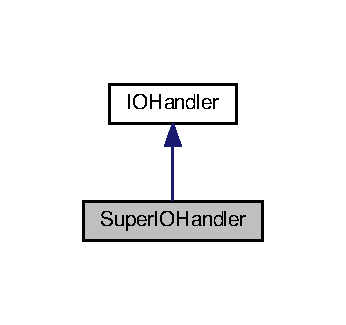
\includegraphics[width=166pt]{classSuperIOHandler__inherit__graph}
\end{center}
\end{figure}


Collaboration diagram for Super\+I\+O\+Handler\+:\nopagebreak
\begin{figure}[H]
\begin{center}
\leavevmode
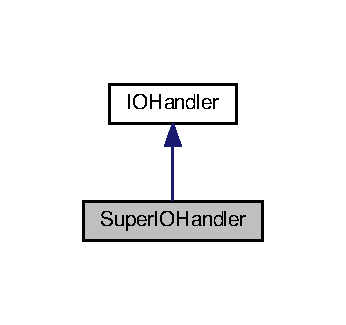
\includegraphics[width=166pt]{classSuperIOHandler__coll__graph}
\end{center}
\end{figure}
\subsection*{Public Member Functions}
\begin{DoxyCompactItemize}
\item 
void {\bfseries on\+Read} (size\+\_\+t fd, fd\+\_\+set $\ast$readfd) override\hypertarget{classSuperIOHandler_ac372c2c513d0118b17d69e2a539c6e43}{}\label{classSuperIOHandler_ac372c2c513d0118b17d69e2a539c6e43}

\item 
void {\bfseries on\+Read} (std\+::shared\+\_\+ptr$<$ \hyperlink{classSocket}{Socket} $>$ \&client, fd\+\_\+set $\ast$readfd) override\hypertarget{classSuperIOHandler_a06246ae2e89c1162f213aa231088c2d3}{}\label{classSuperIOHandler_a06246ae2e89c1162f213aa231088c2d3}

\end{DoxyCompactItemize}


The documentation for this class was generated from the following file\+:\begin{DoxyCompactItemize}
\item 
super.\+cpp\end{DoxyCompactItemize}

%--- End generated contents ---

% Index
\backmatter
\newpage
\phantomsection
\clearemptydoublepage
\addcontentsline{toc}{chapter}{Index}
\printindex

\end{document}
